
\chapter{Excercise 1B:4th order system}
in this assignment a controller wil be designed such that the first mass (m1) from Exercise 0 will respond to the input within reasonable bandwidth.\\
because there is no direct application for the system a bandwidth of 30hz will be used as a rough estimate. this will filter any high frequency disturbances, and the system input will most likely be quite discreet so low frequency\\
in formula \eqref{eq:H1_2} the transfer function is given. this transfer function has to be multiplied with the controller $C(s)=k_p+k_vs$ this results in a large,difficult to solve solution. this means that instead of an analytical approach,Matlab will be used to optimize the controller.

using the matlab pid controller tool a matching kp and kv value are determined.
for a bandwith of 30hz and a phase margin of 60 degrees the values are


	\begin{equation}
K_p=0.5968
	\end{equation}\break
	\begin{equation}
K_d=.003407
	\end{equation}

when optimized for the bandwith of 30hz the overshoot and settling time are larger then for a larger bandwith. this gives the choice between either filtering for disturbance or a more damped system.
\begin{figure}[H] 
	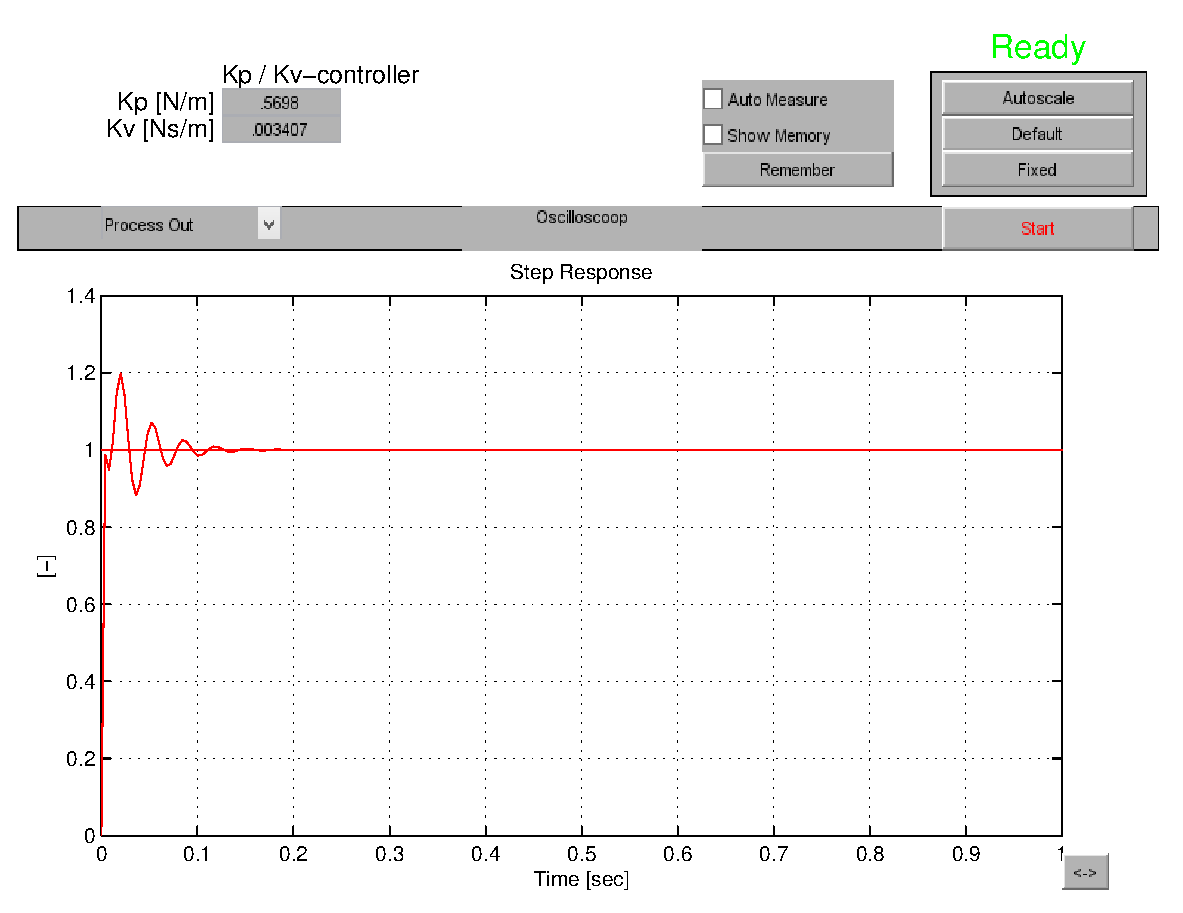
\includegraphics[width=0.8\textwidth]{step30hz.eps}
	\centering
	\caption{step response of the 30hz bandwitdth controller}
	\label{fig:intro_system}
\end{figure}

this settling time is more then .1 seconds.
this is to large considering your input could be 30hz. the system is not settled before the inout changes

